\documentclass{article}
\usepackage{amsmath}
\usepackage{amsfonts}
\usepackage{tikz}
\usepackage{pgfplots}
\usepackage{multicol}

\title{\textbf{Exponential Equations}}\\
\author{Tutoring Centre Ferndale\\

\includegraphics[width=4em]{ApS_logo.png}}
\date{}

\begin{document}

\maketitle

An exponential equation is an equation in which a constant base is raised to a variable exponent. The general form of an exponential equation is:
\begin{center}
{\Large $y = a \cdot b^x$}
\end{center}

where \(a\) is a constant, \(b\) is the base, and \(x\) is the exponent.

\begin{itemize}
    \item If \(b > 1\), the function is increasing.
    \item If \(0 < b < 1\), the function is decreasing.
    \item The function never touches the x-axis: it approaches but never reaches zero.
    \item The y-intercept is at \(y = a\) when \(x = 0\).
\end{itemize}

\section*{Graphing Exponential Equations}
Let's plot the graph of \(y = 2^x\):

\begin{center}
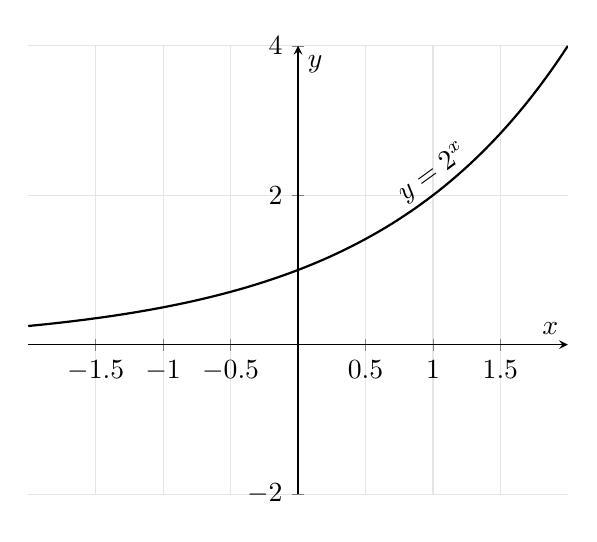
\begin{tikzpicture}
    \begin{axis}
        [axis lines = middle,
        xlabel = {$x$},
        ylabel = {$y$},
        domain=-2:2,
        restrict y to domain=-2:4,
        samples=100,
        ymin=-2, ymax=4,
        xmin=-2, xmax=2,
        grid=both,
        ytick={-2,0,2,4},
        xtick={-1.5,-1,-0.5,0,0.5,1,1.5},
        grid style={draw=gray!20}]
        \addplot[thick] {2^x};
        \node[rotate=36] at (axis cs:1,2.3) {\(y = 2^x\)};
    \end{axis}
\end{tikzpicture}
\end{center}

\subsection*{Effects of Different Values of \(a\)}
Here are the graphs of \(y = a \cdot 2^x\) for different values of \(a\).

\begin{center}
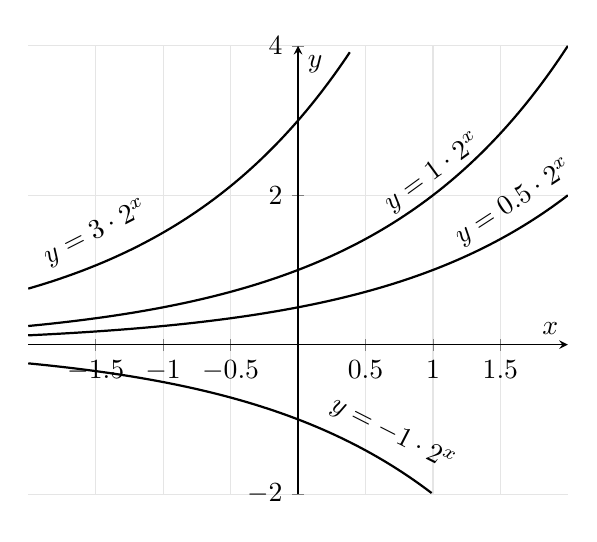
\begin{tikzpicture}
    \begin{axis}
        [axis lines = middle,
        xlabel = {$x$},
        ylabel = {$y$},
        domain=-2:2,
        restrict y to domain=-2:4, % Restrict y values
        samples=100,
        ymin=-2, ymax=4,
        xmin=-2, xmax=2,
        grid=both,
        ytick={-2,0,2,4},
        xtick={-1.5,-1,-0.5,0,0.5,1,1.5},
        grid style={draw=gray!20}]
        
        \addplot[thick] {1*2^x};
        \node[rotate=36] at (axis cs:1,2.3) {\(y = 1 \cdot 2^x\)};
        
        \addplot[thick] {3*2^x};
        \node[rotate=27] at (axis cs:-1.5,1.5) {\(y = 3 \cdot 2^x\)};
        
        \addplot[thick] {0.5*2^x};
        \node[rotate=33] at (axis cs:1.6,1.9) {\(y = 0.5 \cdot 2^x\)};
        
        \addplot[thick] {-1*2^x};
        \node[rotate=-27] at (axis cs:0.7,-1.2) {\(y = -1 \cdot 2^x\)};
    \end{axis}
\end{tikzpicture}
\end{center}

The value of \(a\) affects the vertical stretch or compression and the vertical translation of the graph:
\begin{itemize}
    \item If \(a > 1\), the graph stretches vertically.
    \item If \(0 < a < 1\), the graph compresses vertically.
    \item If \(a < 0\), the graph reflects across the x-axis and then stretches or compresses based on the magnitude of \(a\).
    \item The y-intercept of the graph is at \(y = a\) when \(x = 0\).
\end{itemize}

\newpage

\subsection*{Effects of Different Values of \(b\)}
Here are the graphs of \(y = 2 \cdot b^x\) for different values of \(b\).

\begin{center}
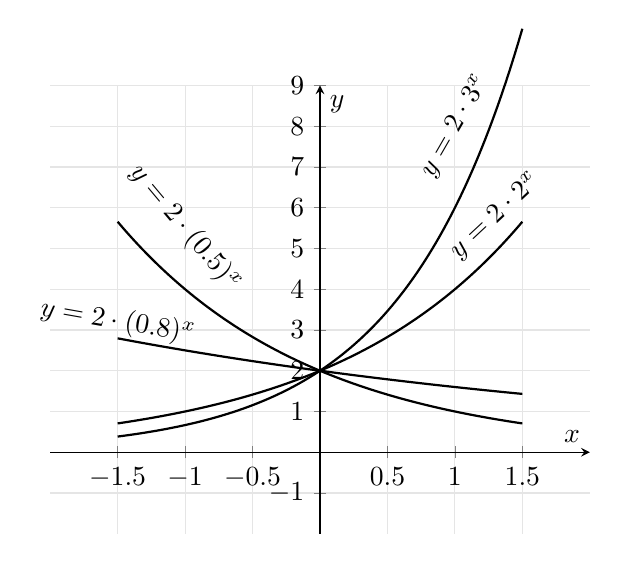
\begin{tikzpicture}
    \begin{axis}
        [axis lines = middle,
        xlabel = {$x$},
        ylabel = {$y$},
        domain=-1.5:1.5,
        samples=100,
        clip=false,
        ymin=-2, ymax=9,
        xmin=-2, xmax=2,
        grid=both,
        ytick={-1,0,1,2,3,4,5,6,7,8,9},
        xtick={-1.5,-1,-0.5,0,0.5,1,1.5},
        grid style={draw=gray!20}]
        \addplot[thick] {2*2^x};
        \node[rotate=43] at (axis cs:1.3,5.8) {\(y = 2 \cdot 2^x\)};
        \addplot[thick] {2*3^x};
        \node[rotate=60] at (axis cs:1,8) {\(y = 2 \cdot 3^x\)};
        \addplot[thick] {2*(0.5)^x};
        \node[rotate=-50] at (axis cs:-1,5.5) {\(y = 2 \cdot (0.5)^x\)};
        \addplot[thick] {2*(0.8)^x};
        \node[rotate=-10] at (axis cs:-1.5, 3.2) {\(y = 2 \cdot (0.8)^x\)};
    \end{axis}
\end{tikzpicture}
\end{center}

The value of \(b\) affects the rate of growth or decay of the graph:
\begin{itemize}
    \item If \(b > 1\), the function is an increasing exponential function, showing exponential growth.
    \item If \(0 < b < 1\), the function is a decreasing exponential function, showing exponential decay.
    \item The base \(b\) determines how rapidly the function increases or decreases:
    \begin{itemize}
        \item Larger values of \(b > 1\) result in steeper growth.
        \item Smaller values of \(0 < b < 1\) result in slower decay.
    \end{itemize}
\end{itemize}

\section*{Practical Uses}
Exponential equations have practical applications, including:
\begin{itemize}
    \item \textbf{Population Growth}: The population of a species or community can be modeled using exponential functions.
    \item \textbf{Radioactive Decay}: The decay of radioactive substances follows an exponential pattern.
    \item \textbf{Interest Calculations}: Compound interest in finance is calculated using exponential functions.
\end{itemize}

\newpage

\section*{Exercises}
\begin{enumerate}
    \item Solve for \(x\): \(2^x = 16\).
    \item Graph the function \(y = 5^{x-2}\).
    \item If a population doubles every 3 years, express the population \(P\) as a function of time \(t\) (in years), given the initial population is \(P_0\).
    \item Solve for \(x\): \(3^{x+1} = 27\).
\end{enumerate}

\subsection*{Answers}

\begin{enumerate}
    \item \(2^x = 16\)\\
    \(16 = 2^4\)\\
    Therefore, \(x = 4\).
    \item The graph of \(y = 5^{x-2}\):
    \begin{center}
    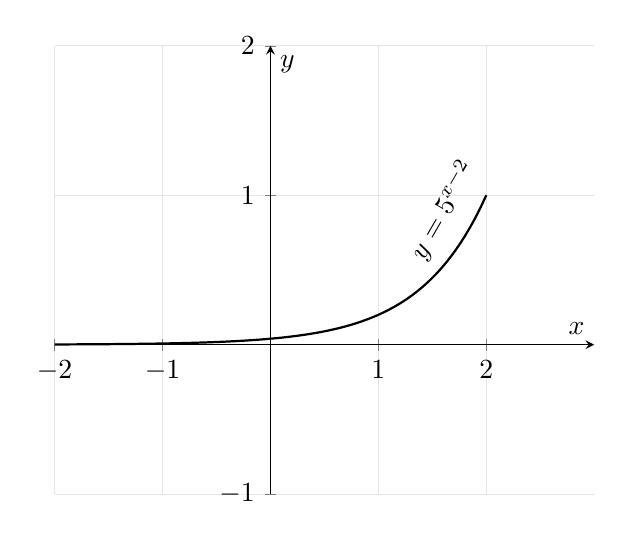
\begin{tikzpicture}
        \begin{axis}
            [axis lines = middle,
            xlabel = {$x$},
            ylabel = {$y$},
            domain=-2:2,
            samples=100,
            ymin=-1, ymax=2,
            xmin=-2, xmax=3,
            grid=both,
            ytick={-1,0,1,2},
            xtick={-2,-1,0,1,2},
            grid style={draw=gray!20}]
            \addplot[thick] {5^(x-2)};
            \node[rotate=60] at (axis cs:1.6,0.9) {$y=5^{x-2}$};
        \end{axis}
    \end{tikzpicture}
    \end{center}
    \item The population \(P\) as a function of time \(t\) can be expressed as:
    \[
    P(t) = P_0 \cdot 2^{t/3}
    \]
    \item \(3^{x+1} = 27\)\\
    \(27 = 3^3\)\\
    Therefore, \(x + 1 = 3\)\\
    \(x = 2\).
\end{enumerate}

\end{document}
